% Separado de setup-hardware.tex em 2026-11-04: as ferramentas e o módulo ficam antes
%   (ferramentas); as arquiteturas, as matrizes de teste e a potência vêm depois do formato.
The chosen formats were synthesized using Vitis HLS. In all versions, the automatic loop pipelining feature was disabled \cite[p.~42]{ug1399}. The first version, without loop optimizations, was implemented for both $16 \times 16$ and $32 \times 32$ matrix sizes. In this version, the iterations of each loop execute sequentially, and the $N_{\text{PRB}} = 275$ matrices within a block are inverted one by one. Consequently, the interval between inversions exceeds the limits defined for all test conditions (Table~\ref{tab:limite-ciclos}), and the module does not track the arrival of the matrices at each $T_c$.

To meet the cycle limits for each test condition, a specific architecture was developed for every case, only in $16 \times 16$, with Vitis HLS directives that reduce the interval between inversions. All versions were implemented in Vivado, tested using $\mathbf G_c$ matrices obtained from the simulator (Section~\ref{subsec:hw-matrizes}), and evaluated for power consumption and energy per inversion (Section~\ref{subsec:hw-potencia}). Each version produces the same inverse as the non-optimized implementation, a result verified bit-for-bit against the C-language code.
% FONTE: hardware/viabilidade_32x32/LEIAME.md (síntese C, HLS 2026.1 local, 2026-11-02, <24,12>).
\textcolor{red}{As arquiteturas otimizadas não foram implementadas em $32 \times 32$. Uma síntese C de teste das seis, em $32 \times 32$ e no formato $\langle 24,12\rangle$, estimou intervalos acima do limite de ciclos de todas as condições de teste. Nas sistólicas, o intervalo cresce 4 vezes, com o quadrado do tamanho da matriz. A da TDLB100-400 também não caberia no FPGA. Para atender os limites em $32 \times 32$, seria preciso outra arquitetura, com mais área, e isso não foi testado.}

\subsection{\texorpdfstring{Hardware architectures}{Hardware architectures}}\label{subsec:hw-arquiteturas}
% ---------------------------------------------------------------------
All optimized architectures employ pipelining (Section~\ref{subsubsec:latencia-intervalo}). Every $T_c$, the DU inverts 275 matrices $\mathbf G_c$, one for each PRB (Section~\ref{sec:requisitos-tempo}). For the 9,090 and 4,545-cycle limits, the module inverts one matrix at a time. For tighter limits, it inverts the matrices in batches of $n$. In all cases, the module must receive the 275 matrices for a given block within the duration $T_c$.

The matrices within a batch are independent of one another. Consequently, $c$ of these matrices are computed in the same cycle using loop unrolling, which creates a copy of the loop body for each iteration. The loop that iterates over the $c$ matrices is nested within a pipelined loop, and the HLS tool performs the unrolling automatically \cite[pp.~41, 372, and 428]{ug1399}. When $c$ is less than $n$, groups of $c$ matrices are processed in alternating cycles. Each copy has its own dedicated memory bank, though it may share operators with the others.

The values for $n$ and $c$ were determined through trial and error and are presented in Table~\ref{tab:hw-arquiteturas}.
 

\begin{table}[htbp]
\caption{Batch of the inversion module in each test condition.}
\label{tab:hw-arquiteturas}
\vspace{4pt} % a classe zera o espaço entre a caption e a tabela
\centering
\footnotesize

\renewcommand{\arraystretch}{1.2}
\setlength{\tabcolsep}{4pt}
\begin{tabular}{lcccc}
\toprule
\textbf{Test condition} & \begin{tabular}[c]{@{}c@{}}\textbf{Limit per}\\\textbf{matrix (cycles)}\end{tabular} & \begin{tabular}[c]{@{}c@{}}\textbf{Matrices per}\\\textbf{batch} ({\boldmath $n$})\end{tabular} & \begin{tabular}[c]{@{}c@{}}\textbf{Copies}\\({\boldmath $c$})\end{tabular} & \begin{tabular}[c]{@{}c@{}}\textbf{Batches}\\\textbf{per block}\end{tabular} \\
\midrule
Without optimizations & --    & 1  & 1 & 275 \\
TDLA30-5    & 9090 & 1  & 1 & 275 \\
TDLA30-10   & 4545 & 1  & 1 & 275 \\
TDLA30-75   & 606   & 12 & 6 & 23 \\
TDLC300-100 & 454   & 16 & 8 & 18 \\
TDLA30-300  & 151   & 32 & 2 & 9 \\
TDLB100-400 & 113   & 32 & 4 & 9 \\
\bottomrule
\end{tabular}

\vspace{4pt}
\legend{Source: the author. Limit per matrix from Table~\ref{tab:limite-ciclos}.}
\end{table}



% ---------------------------------------------------------------------
\subsubsection{\texorpdfstring{Loop pipelining}{Loop pipelining}}\label{subsubsec:hw-pipeline-lacos}

The module consists of six sequential stages (Figure~\ref{fig:modulo-inversao}): LU decomposition, extraction of the diagonal $\mathbf D$, calculation of the square root $\mathbf D^{1/2}$, computation of $\mathbf F$, forward substitution, and inversion. For the 9,090-cycle limit, the internal loops of these stages are annotated with the \texttt{\#pragma HLS pipeline II=1} directive. The \texttt{D\_extraction} stage is the only one without this directive, as it merely copies the diagonal from $\mathbf U$ to $\mathbf D$ and requires significantly fewer cycles than the other stages.

This directive enables loop pipelining, specifying that a new iteration should begin every cycle, that is, an initiation interval (II) of 1 cycle (Section~\ref{subsubsec:latencia-intervalo}). If data dependencies or resource constraints prevent this, the HLS tool will automatically use a larger II \cite[p.~45]{kastner-hls}.

Figure~\ref{fig:hw-pipeline-lacos} illustrates a loop from the LU decomposition process, both without and with pipelining. The individual stages and loops for a given matrix are executed sequentially. Consequently, the next inversion process cannot begin until the current one has finished; in this case, the interval between inversions is equal to the latency \cite[p.~114]{kastner-hls}.

\begin{figure}[!ht]
\caption{Loop pipelining in the LU decomposition. The code is simplified.}
\label{fig:hw-pipeline-lacos}
\vspace{4pt} % a classe zera o espaço entre a caption e a figura
\centering
\begin{minipage}[c]{0.62\textwidth}
\fontsize{8}{9.6}\selectfont
\begin{verbatim}
for (line = column + 1; line < n; line++)
  for (k = column; k < n; k++) {
#pragma HLS pipeline II=1
    t = L[line][column] * U[column][k];
    U[line][k] = U[line][k] - t;
  }
\end{verbatim}
\end{minipage}

\vspace{8pt}
\begin{minipage}[c]{\textwidth}
\centering
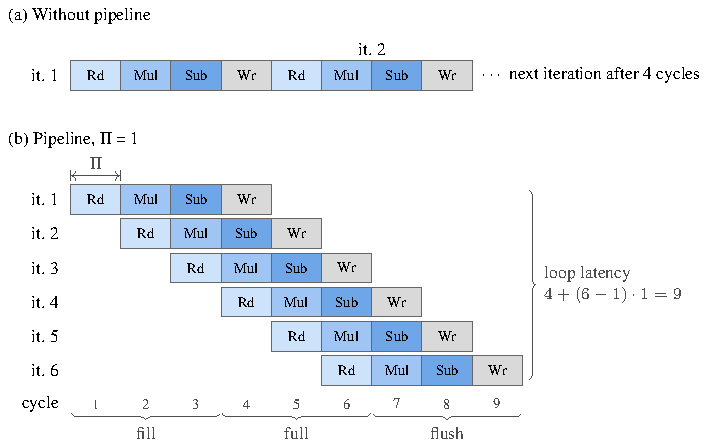
\includegraphics{Images/FLUXO/hw_pipeline_lacos.pdf}
\end{minipage}
\vspace{4pt}
\legend{Source: the author. Rd: read, Mul: multiply, Sub: subtract, Wr: write. Iteration latency of 4 cycles, for illustration.}
\end{figure}

% ---------------------------------------------------------------------
\subsubsection{\texorpdfstring{Dataflow between stages}{Dataflow between stages}}\label{subsubsec:hw-dataflow}

The architecture of the 4,545-cycle limit maintains the loop pipeline and combines the six steps into four: LU decomposition, calculation of $\mathbf F$ (\texttt{D\_extraction}, \texttt{D\_square\_root} and \texttt{G\_decomposition}), forward substitution, and inversion. The \texttt{\#pragma HLS dataflow} directive, applied to the top-level function, implements a task-level pipeline across the four stages, with each stage assigned to a specific matrix (Section~\ref{subsubsec:pipeline-tarefas}). Each step carries the directive \texttt{\#pragma HLS inline off}, which keeps it as a separate function \cite[p.~52]{kastner-hls}. In Figure~\ref{fig:hw-dataflow}, the latency of a matrix is the sum of the four steps, and the interval is the duration of the longest step.

% FONTE: cholesky_hardware_diretivas_4545/cholesky_top.cpp (etapa_lu, etapa_g, etapa_fs,
%   etapa_inv; dataflow em cholesky_inverse, linha 68). Kastner p. 52 (inline off mantém a
%   hierarquia), p. 114 (dataflow: as funções executam ao mesmo tempo, em dados diferentes).
%   Intervalo = etapa mais longa: Kastner p. 115 (na Fundamentação).

\begin{figure}[!ht]
\caption{Dataflow between the stages of the inversion. The code is simplified.}
\label{fig:hw-dataflow}
\vspace{4pt}
\centering
\begin{minipage}[c]{0.45\textwidth}
\fontsize{8}{9.6}\selectfont
\begin{verbatim}
void cholesky_inverse(A, inverse) {
#pragma HLS dataflow
  etapa_lu(A, L, U);
  etapa_g(U, L, G);
  etapa_fs(G, G_inv);
  etapa_inv(G_inv, inverse);
}

static void etapa_fs(G, G_inv) {
#pragma HLS inline off
  forward_substitution(G, G_inv);
}
\end{verbatim}
\end{minipage}

\vspace{8pt}
\begin{minipage}[c]{\textwidth}
\centering
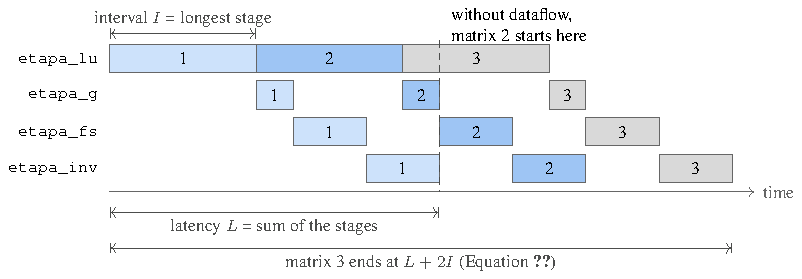
\includegraphics{Images/FLUXO/hw_c2.pdf}
\end{minipage}
\vspace{4pt}
\legend{Source: the author. Numbers in the boxes: index of the matrix.}
\end{figure}

% ---------------------------------------------------------------------
\subsubsection{\texorpdfstring{Matrix batches}{Matrix batches}}\label{subsubsec:hw-lotes}


Within the 606 and 454 cycle limits, the steps form a dataflow, as in the 4,545 cycle limit. The $c$ copies read different matrices in the same cycle, but a BRAM memory only allows access to two addresses per cycle. Therefore, the batch memory is divided into $c$ BRAM banks, one per copy, using the directive \texttt{\#pragma HLS array\_partition cyclic} and factor $c$. Thus, matrix $m$ is located in bank $m \bmod c$ \cite[pp.~87--88]{kastner-hls}.

Figure~\ref{fig:hw-lotes} shows the architecture of the 606 cycle limit. Since the two groups of 6 matrices alternate in each cycle, one iteration does not wait for the result of the previous one. Each copy has its own multipliers, but there is a single divider in each step, shared by the copies. It receives one matrix of the batch per cycle and, since it has a pipeline, it also does not wait for the previous division.

\begin{figure}[!ht]
\caption{Batch of 12 matrices with 6 copies, for the 606-cycle limit. The code is simplified.}
\label{fig:hw-lotes}
\vspace{4pt}
\centering
\begin{minipage}[c]{0.62\textwidth}
\fontsize{8}{9.6}\selectfont
\begin{verbatim}
#pragma HLS array_partition variable=U \
                     cyclic factor=COPIES dim=1
for (k = column; k < n; k++)
  for (g = 0; g < GRUPOS; g++) {
#pragma HLS pipeline II=1
    for (p = 0; p < COPIES; p++) {
      m = g * COPIES + p;
      t = L[m][line][column] * U[m][column][k];
      U[m][line][k] = U[m][line][k] - t;
    }
  }
\end{verbatim}
\end{minipage}

\vspace{8pt}
\begin{minipage}[c]{\textwidth}
\centering
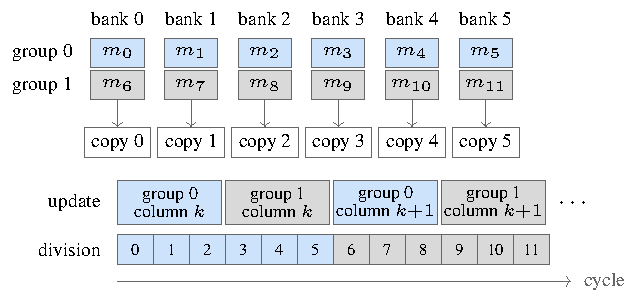
\includegraphics{Images/FLUXO/hw_c3.pdf}
\end{minipage}
\vspace{4pt}
\legend{Source: the author. Bank $p$ holds the matrices with $m \bmod 6 = p$. Update: 6 matrices per cycle. Division: one matrix $m$ per cycle, in a single divider.}
\end{figure}

% ---------------------------------------------------------------------
\subsubsection{\texorpdfstring{Systolic arrays}{Systolic arrays}}\label{subsubsec:hw-sistolico}

Within the 151 and 113-cycle limits, the stages also form a dataflow, with each copy featuring its own divider. LU decomposition, forward substitution, and inversion utilize systolic arrays: the $k$-loop, which iterates over a row or a summation, is nested within a pipelined loop, which HLS unrolls into 16 processing elements (PEs) (Section~\ref{subsubsec:arranjo-sistolico}). Each stage employs an array structure per copy, resulting in a total of $3c$ such arrays within the module.

In forward substitution and inversion, each PE adds a term and passes the partial sum to the next PE, following the same sequence as the unoptimized version, with each cycle computing a complete sum. In the LU decomposition, each cycle updates an entire row, with one element assigned to each PE. To achieve this, each row element is stored in its own dedicated register, configured using the \texttt{\#pragma HLS array\_partition complete} directive \cite[p.~87]{kastner-hls}.

In both LU decomposition and forward substitution, each step reads rows that were written during the previous step, with a cycle offset corresponding to the step size. During the final steps of the LU decomposition and the initial steps of the forward substitution, which are relatively short, the required row might still be within the pipeline. Consequently, these steps are padded with empty cycles until they reach a minimum duration (Figure~\ref{fig:hw-sistolico}). Since HLS cannot automatically infer this from the source code, the \texttt{\#pragma HLS dependence ... dependent=false} directive is used to specify that the iterations are independent of one another \cite[p.~149]{kastner-hls}.


\begin{figure}[!ht]
\caption{Systolic array of the forward substitution and minimum step of the LU decomposition. The code is simplified.}
\label{fig:hw-sistolico}
\vspace{4pt}
\centering
\begin{minipage}[c]{0.62\textwidth}
\fontsize{8}{9.6}\selectfont
\begin{verbatim}
#pragma HLS array_partition variable=Ua \
                     complete dim=3
for (it = 0; it < LU_ITER; it++) {
#pragma HLS pipeline II=1
#pragma HLS dependence variable=Ua \
          type=inter dependent=false
  if (idx < reais)       // else: empty
    for (p = 0; p < COPIES; p++)
      for (k = 0; k < n; k++)  // PEs
        Ua[m][line][k] = row[k] - l*piv[k];
}
\end{verbatim}
\end{minipage}

\vspace{8pt}
\begin{minipage}[c]{\textwidth}
\centering
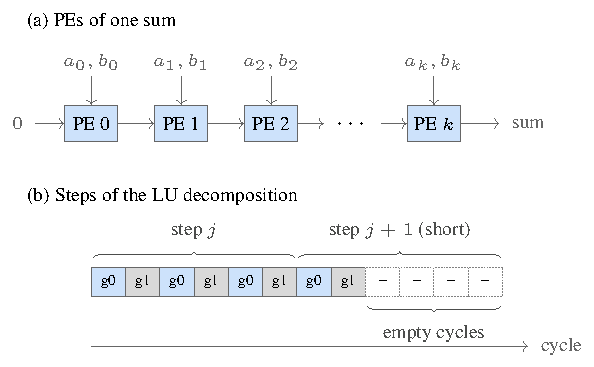
\includegraphics{Images/FLUXO/hw_c4.pdf}
\end{minipage}
\vspace{4pt}
\legend{Source: the author. g0, g1: groups of matrices of the batch, one per cycle; there are 16 groups for the 151-cycle limit and 8 for the 113-cycle limit.}
\end{figure}

% ---------------------------------------------------------------------
\subsection{\texorpdfstring{Test matrices}{Test matrices}}\label{subsec:hw-matrizes}
% ---------------------------------------------------------------------
The hardware was tested with the same $\mathbf{G}_c$ matrices that BCD-MMSE inverts in the SER curves, with 1 iteration. These matrices were saved before inversion, in each of the 5 distinct test conditions (Section~\ref{subsec:setup_condicoes}). In each condition, a sample was saved: some matrices randomly selected by configuration and SNR point, and the most extreme in range and precision, such as those with the largest element and the largest condition number. QPSK configurations were excluded because the modulation does not change $\mathbf{G}_c$.

The testbench inverts 20 matrices randomly selected from this sample. In the $16 \times 16$ circuit, these matrices come only from configurations 1A--1H. In architectures with batch, the 20 matrices are repeated until at least 3 batches are completed.


% FONTE: rodar_potencia.py (sinteses/*_vivado/potencia/): 20 matrizes sorteadas com
%   semente fixa; 16x16: 1A, 1B, 1E e 1F; 32x32: 2A, 2B, 2E e 2F; grupo 3 fora da potência
%   (decisão da autora). tb_potencia.cpp da 606 (linhas 57-71: lotes = max(3, ceil(20/LOTE)));
%   potencia.csv: 36 (606), 48 (455), 96 (152 e 114), 20 nas outras.

% ---------------------------------------------------------------------
\subsection{\texorpdfstring{Power and energy}{Power and energy}}\label{subsec:hw-potencia}
% ---------------------------------------------------------------------
Power was estimated from the switching activity of the routed design: the version without optimizations under the 5 test conditions, and each optimized architecture only under its own. Vivado generates a functional netlist, which is simulated with the testbench. The simulation checks the inverses byte by byte against the C code and records how many times each signal changes value in a SAIF (Switching Activity Interchange Format) file. Vivado then reads this file and reports the power.

Energy per inversion is defined as the dynamic power multiplied by the average time required for an inversion. This duration is calculated as the interval between two inversions, measured during the netlist simulation, multiplied by the 10~ns clock period. In architectures that employ batch processing, the interval between two batches is divided by $n$.
\textcolor{red}{A potência estática é a potência total menos a dinâmica.}
% Retirado em 2026-11-13 (a figura potencia_media_condicao saiu dos Resultados em 2026-11-09):
%   A potência média no ritmo exigido de cada condição de teste soma a potência estática e a
%   energia de 275 inversões dividida por T_c. Ela supõe que, depois de inverter as 275 matrizes
%   do bloco, o módulo fica parado até o próximo bloco e só gasta a potência estática.
% FONTE: memória tcc-pacote-servidor-2023 (convenção da energia). Intervalo tirado do
%   xsim_<cenário>.log do servidor, não do ciclos_medios do potencia.csv, que inclui o
%   enchimento do pipeline do primeiro lote.
